\documentclass[12pt, a4paper, oneside]{ctexbook}
\usepackage{amsmath, amsthm, amssymb, bm, graphicx, hyperref, mathrsfs, mhchem, geometry}
\geometry{left = 3.7cm, right = 3.2cm, top = 3cm, bottom = 3cm}

\title{{\Huge{\textbf{基础化学}}}\\笔记}
\author{F1}
\date{\today}
\linespread{1.5}
\newtheorem{theorem}{定理}[section]
\newtheorem{definition}[theorem]{定义}
\newtheorem{lemma}[theorem]{引理}
\newtheorem{corollary}[theorem]{推论}
\newtheorem{example}[theorem]{例}
\newtheorem{proposition}[theorem]{命题}

\begin{document}

\maketitle

\pagenumbering{roman}
\setcounter{page}{1}

%\begin{center}
%    \Huge\textbf{前言}
%\end{center}~\

%这是笔记的前言部分. 
%~\\
%\begin{flushright}
%    \begin{tabular}{c}
%        Dylaaan\\
%        \today
%    \end{tabular}
%\end{flushright}

%\newpage
\pagenumbering{Roman}
\setcounter{page}{1}
\tableofcontents
\newpage
\setcounter{page}{1}
\pagenumbering{arabic}

\chapter{准备知识}


\section*{有效数字}
从第一个不为零的数字算起的所有数字。\\
0.06050为四位有效数字\\
单位变换不能影响有效数字。例:10.00mL -> 0.001000L 均为四位有效数字\\
注意:pH = 11.20 表示 [$H^+$]=6.3 * 10$^{-12}$为两位有效数字。\\
有效数字的意义:既能表达数值大小,又能表明测量值准确程度的数字的表示方法,
它包括测得的全部准确数字和一位可疑数字,可疑数字的误差內为+-1。刻度型仪器的测量值,最后一位数字是估计的,因此是可疑数字。\\
\subsection*{有效数字的修约规则}
\begin{enumerate}
    \item 四舍六入五成双(后面一位数字为5时)5前奇数进位,偶数舍去。\\例:1.15->1.2 1.25->1.2
    \item 若5后有非零数字,则5进位。\\例:1.151->1.2
    \item 
\end{enumerate}

\subsection*{有效数字的运算法则}
只对最后结果进行修约。
\begin{enumerate}
    \item 加减法:结果小数点后保留最少位数的有效数字。\\例:50.1+1.45+0.5812 = \textbf{52.1}
    \item 乘除法:以有效数字位数最少的数字为准。\\例:0.0121 * 25.64 * 1.05782 = 0.32818231 = \textbf{0.328}
    \item 加减乘除混合运算:3.489 * (5.67 - 2.3) = 3.489 * 3.37(先不修约) = 11.75793 = 11.758 = \textbf{12}\\6.78 * 5.903 * (5.489 - 5.01) = 6.78 * 5.903 * 0.479 = 19.1707 = \textbf{19}\\
    \item 
\end{enumerate}

\subsection*{小结}
\begin{enumerate}
    \item 有效数字的意义:注意对数与幂形式的转化(pH与浓度)
    \item 有效数字的修约:4舍6入5成双
    \item 
\end{enumerate}

\textbf{只对最后结果进行修约}



\section*{混合物的组成标度}
\begin{enumerate}
    \item 质量分数$w$ \\某溶质质量与混合物质量之比:$w = \frac{m_s}{m}$
    \item 体积分数$\varphi$\\在某一温度下,溶质体积与混合物体积之比:$\varphi = \frac{V_s}{V}$
    \item 摩尔分数$x$ 某溶质
    \item 质量浓度$\rho $
    \item 物质的量浓度$c$(与温度有关)\\溶液中溶质B的物质的量$n_B$与溶液体积之比:$c_B = \dfrac{\text{溶质B的物质的量(mol)}}{\text{溶液的体积}}$\\
            单位 mol$\cdot$m$^{-3}$, mol$\cdot$L$^{-1}$.\\
            注:使用$c_B$必须指明基本单元,对于具体物质,应将基本单元表示在括号内如$c_{\text{NaCl}}$,对于溶液,应将溶剂表示在括号内如$c_{\text{(Ca$^{2+}$)}} = 2$mmol$\cdot$L$^{-1}$
    \item 质量摩尔浓度$b$ (与温度无关)\\单位 mol$\cdot$ kg$^{-1}$\\
            溶液中溶质B的物质的量$n_B$与溶液质量之比:$b_B = \dfrac{\text{溶质B的质量(kg)}}{\text{溶液的质量(kg)}}$\\
\end{enumerate}
例题:将7.00g草酸晶体()溶解于93.0g水中,求草酸的摩尔质量浓度$b(\ce{H2SO4})$和摩尔分数$x$.\\

\chapter{稀溶液的依数性}
背景内容
\begin{enumerate}
    \item 溶液的蒸汽压
    \item 溶液的沸点、凝固点
    \item 溶液的渗透压力
\end{enumerate}
\newpage
\section{溶液的基本问题}
温度与压力共同决定物质的形态。\\
\begin{figure}[htbp]
    \centering
    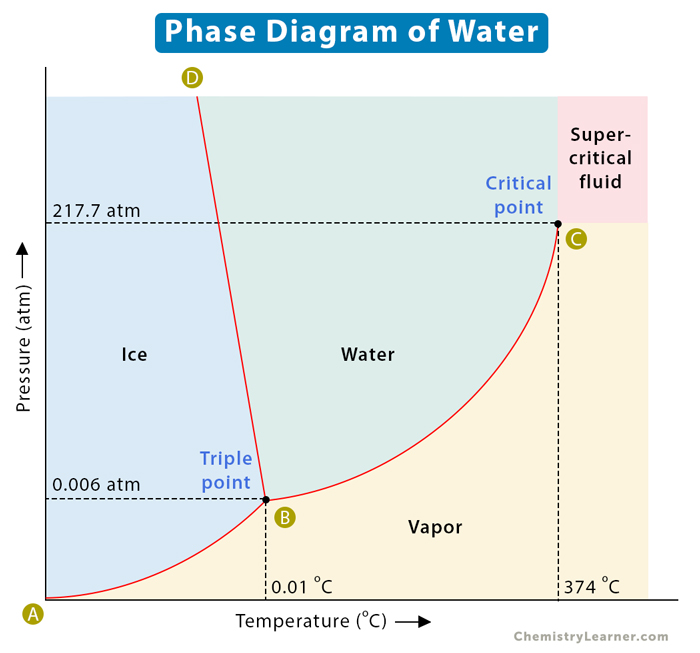
\includegraphics[width=0.8\textwidth]{pics/phase_diagram.jpg}
    \caption{水的相图}
\end{figure}
\subsection{气液平衡:液体的蒸发、蒸汽压}
\subsubsection{蒸发}
液体从周围环境中吸收热量,分子动能增加,部分表层分子克服分子间引力,逃逸出液面,形成气体。\\
\subsubsection{凝结}
密闭容器中,随着蒸发的进行,由液面溢出的蒸气分子在相互碰撞过程中,部分分子返回液相,这个过程叫凝结。\\
\subsubsection{饱和蒸气压}
一定温度下,密闭容器中,当液体蒸发与凝结达到动态平衡时,液体表面上的蒸气与液体之间的相互转化达到平衡。此时蒸汽压不再增大,为一定值,叫做饱和蒸气压,简称蒸汽压($p$)。\\
\subsubsection*{蒸汽压与液体的本性和温度密切相关}
一定温度下,液体的蒸汽压是一个定值,与气体的体积、液相的量无关,只与液体的本性和温度密切有关。
\begin{figure}[htbp]
    \centering
    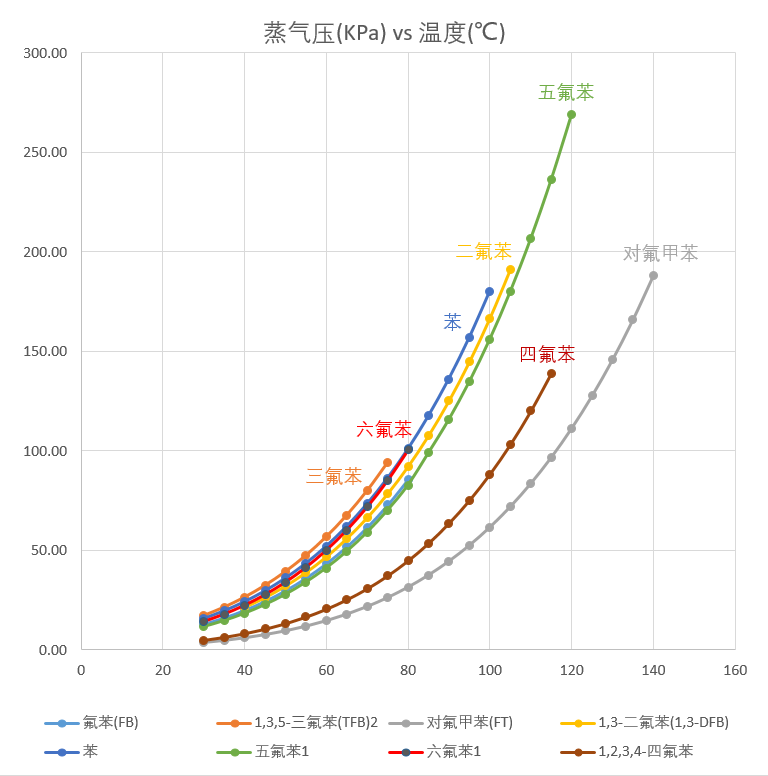
\includegraphics[width=0.8\textwidth]{pics/vapor_pressure.png}
    \caption{蒸汽压-温度曲线}
\end{figure}

\newpage
\subsubsection{液体的沸腾与沸点}
在敞开体系,升高温度,液体内部会形成气泡,当气泡的饱和蒸气压等于外部施予的压强时,液体内部的气泡就长大并上升,液体就会沸腾。\\
\subsubsection{液固平衡:液体的凝固、固体的熔化}
凝固点:在一定压强下,液体凝固成固体的温度。\\
从相图来看,在一定压力下,物质的液相和固相蒸汽压相等、两相平衡共存的温度,就是凝固点,用$T_f$ (freezing point)表示。\\

\subsubsection{蒸汽压的注意要点}
\begin{enumerate}
    \item 液体的蒸汽压与温度有关,与液体的量无关。
    \item 蒸汽压与外界大气压相等时,液体沸腾。
    \item 蒸汽压大的称为挥发性液体,蒸汽压小的称为不挥发性液体。
    \item 
\end{enumerate}


溶液:两种或两种以上的物质混合在一起,形成的均匀稳定分散的体系。
\begin{table}[htbp]
    \centering
    \begin{tabular}{|c|c|c|}
        \hline
         分类方法 & 1 & 2\\
        \hline
        溶质 & 电解质溶液 & 非电解质溶液\\
        \hline
        浓度 & 浓溶液 & 稀溶液\\
        \hline
    \end{tabular}
\end{table}
\\从最简单的体系入手:难挥发、非电解质、稀溶液



\end{document}